\chapter{Experimental results}\label{ch:experiments}

We have four different optimization algorithms to choose from:
\begin{itemize}
    \item \textit{EVO-STOPS} - an evolutionary algorithm that encodes a solution as a list of routes of stops and tries to improve the solution by modifying these routes.
    \item \textit{EVO-CR} - an evolutionary algorithm that encodes a solution using a mapping from groups from buses and an array defining the order of pick-ups and drop-offs.
    \item \textit{EVO-H} - an evolutionary algorithm that uses only the mapping from groups to buses and creates routes using a greedy heuristic.
    \item \textit{ACO-HCF} - iteratively creates new solutions using the \textit{(Hyper-Cube Framework) Ant Colony Optimization} metaheuristic.
\end{itemize}

To compare the approaches, we generated benchmark datasets and ran all the algorithms on them. In this chapter, we present the results.

\section{General parameters}

Some dataset parameters are the same for all used datasets. Each group has between 1 and 10 people. The depot is always set in Prague. It is important to note that the first group in each route gets always picked up on time. This means that the location of the depot has no effect on the group's delays; setting it far from the departure area does, however, make using more buses more costly.

All the algorithms use the same fitness function, with the delay penalty constant equaling $0.01$. All genetic algorithms have $10\%$ of the population's best individuals (\textit{elites}) passed from the old to the new population. Other parameters are set as described in Sections \ref{sec:genetic_hyperparams} and \ref{sec:aco_hyperparams}.

All the genetic algorithms can limit the number of buses used by a hyperparameter. However, the \textit{ACO} does not have this option, as it generates the routes until all customer requests are satisfied. Therefore, all the limits on the number of buses set for each experiment apply only to the generic algorithms.

All experiments were performed on an AMD EPYC 7532 processor. Each algorithm ran for a fixed amount of time before being terminated, and the time of each experiment can be seen in the fitness plots.

For all experiments, we include a plot showing the progression of the best fitness value found by each approach. The value shown is the mean best fitness of 10 different runs, with the first and third quartiles depicted by the translucent region. The figure shows progression in time and has both the x and y axis on a logarithmic scale. The statistics about the best solutions returned by each algorithm are described in two tables. First shows the basic information: total costs (in thousands), kilometers traveled in total, size of the delay penalties in the fitness function (in thousands) and how much of the fitness value they take, and the number of buses used. The second table shows information about group delays - the maximum delay of a group and the average and median delays of all groups, respectively.

\section{Commute dataset}

In the commute dataset, 100 different customer groups depart from a random location in Pilsen and travel to a random location in Prague. The distance between the two cities is approximately 90 km. The departure times are randomly distributed in a four-hour time window. The available bus type can carry up to $80$ people, its operating cost per kilometer is $80$, and its fixed rental cost is $50000$. The algorithms ran for exactly 90 minutes, after which they were terminated.

\subsubsection{30 buses}

When setting the bus limit (for generic algorithms) to 30, we see that the \textit{ACO} performed the worst, since it failed to minimize the number of buses used. This resulted in the highest total costs and the greatest number of kilometers traveled. All genetic algorithms returned similar results. \textit{EVO-CR} minimized the total costs the most while \textit{EVO-H} handled the group delays slightly better.

We can compare the results to a situation where every group would use its own vehicle. The total distance traveled by all groups, from their departure points to their destinations, is 10,112 km. All the genetic algorithms found solutions that reduced the total distance traveled. However, the \textit{ACO} used more buses, resulting in a higher total distance traveled. It is important to note that the buses start from a depot in one city, pick up the groups, drive to another city, and then return to the original depot. Therefore, each bus travels between the cities twice. If we had a two-way commute scenario, where we would use the same buses to return the customers back to their original city, the savings would be much more significant.

\subsubsection{20 buses}

We can try lowering the total costs by limiting the number of buses even more. The results of the \textit{ACO} algorithm stay the same, as the limit does not apply to it. The solutions' fitness value is much more similar than in the previous experiment. However, the characteristics of the solutions are different. \textit{EVO-CR} performed the best out, with the lowest total costs and distance traveled overall, and lowest delays out of all the genetic algorithms. The \textit{EVO-H} solution is very similar. Both the maximum and average delay are nearly double the amount when the bus limit was set to 30. Even though the fitness values are higher for the lower number of buses limit, the solution is not strictly worse.

\clearpage

\begin{figure}
    \centering
    \includegraphics[width=1\linewidth]
    {img/exp_commute_100_time.pdf}
    \caption{Commute dataset, 30 buses limit - Fitness values in time}
    \label{fig:exp_commute_30}
\end{figure}

\begin{table}
    \centering
    \begin{tabular}{lcccccc}
         & Total costs & Distance traveled & Delay penalties & Buses used \\
         \hline
         EVO-STOPS & 2149 & 8732 km & 612 (22\%) & \textbf{29} \\
         EVO-CR & \textbf{2140} & \textbf{8626 km} & 524 (20\%) & \textbf{29} \\
         EVO-H & 2240 & 9255 km & \textbf{429 (16\%)} & 30 \\
         ACO-HCF & 2822 & 12147 km & 472 (14\%) & 37 \\
    \end{tabular}
    \caption{Commute dataset, 30 buses limit - Route statistics}
    \label{tab:exp_commute_30_route_stats}
\end{table}

\begin{table}
    \centering
    \begin{tabular}{lcccccc}
         &  Maximum delay & Average delay & Median delay \\
         \hline
         EVO-STOPS & 30m25s & 11m26s & 11m21s \\
         EVO-CR & 28m2s & 10m10s & 10m26s \\
         EVO-H & \textbf{23m3s} & 9m5s & 8m56s \\
         ACO-HCF & 37m2s & \textbf{7m36s} & \textbf{5m1s} \\
    \end{tabular}
    \caption{Commute dataset, 30 buses limit - Delay statistics}
    \label{tab:exp_commute_30_delay_stats}
\end{table}

\clearpage

\begin{figure}
    \centering
    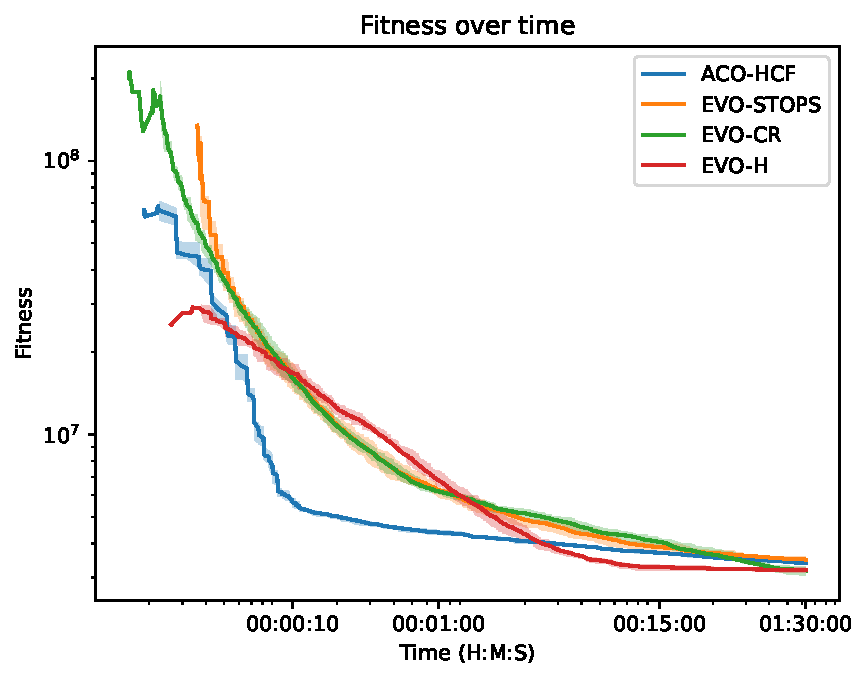
\includegraphics[width=1\linewidth]
    {img/exp_commute_100_20_time.pdf}
    \caption{Commute dataset, 20 buses limit - Fitness values in time}
    \label{fig:exp_commute_20}
\end{figure}

\begin{table}
    \centering
    \begin{tabular}{lcccccc}
         & Total costs & Distance traveled & Delay penalties & Buses used \\
         \hline
         EVO-STOPS & 1629 & 7233 km & 1604 (50\%) & 21 \\
         EVO-CR & \textbf{1552} & \textbf{6900 km} & 1464 (49\%) & \textbf{20} \\
         EVO-H & 1554 & 6927 km & 1472 (49\%) & \textbf{20} \\
         ACO-HCF & 2822 & 12147 km & \textbf{472 (14\%)} & 37 \\
    \end{tabular}
    \caption{Commute dataset, 20 buses limit - Route statistics}
    \label{tab:exp_commute_20_route_stats}
\end{table}

\begin{table}
    \centering
    \begin{tabular}{lcccccc}
         &  Maximum delay & Average delay & Median delay \\
         \hline
         EVO-STOPS & 51m54s & 17m3s & 16m0s \\
         EVO-CR & 42m22s & 17m19s & 16m58s \\
         EVO-H & 44m41s & 17m32s & 16m27s \\
         ACO-HCF & \textbf{37m2s} & \textbf{7m36s} & \textbf{5m1s} \\
    \end{tabular}
    \caption{Commute dataset, 20 buses limit - Delay statistics}
    \label{tab:exp_commute_20_delay_stats}
\end{table}

\clearpage

\section{Uniformly distributed dataset}

\subsection{100 customers}

The uniformly distributed data set has both departure and destination points scattered randomly throughout Prague, and departure times are also randomly distributed within a 5-hour time window. The available bus type can carry up to $40$ people, its operating cost per kilometer is $60$, and its fixed rental cost is $30000$. The wall time was set to 90 minutes.

\subsubsection{25 buses}

When the upper limit of buses for genetic algorithms is set to $25$, the \textit{ACO} clearly outperforms all other approaches, as the limit is set too high. \textit{EVO-CR} struggled the most with lowering the buses used, resulting in the highest overall costs. We can also see that \textit{EVO-STOPS} fails the most in dealing with delay penalties, which are higher than for the \textit{ACO} while using $5$ more buses. \textit{EVO-H} found a solution with minimal group delays, with the maximum delay being under 4 minutes.

\subsubsection{16 buses}

Lowering the upper limit for buses to 16 greatly improves the performance of all genetic algorithms. However, the \textit{ACO} still managed to minimize the total costs the most. \textit{EVO-STOPS} performed the worst in all aspects. \textit{EVO-CR} and \textit{EVO-H} performed similarly, with \textit{EVO-CR} using a bus more, but having slightly shorter delays. The \textit{ACO} run is the same as in the previous experiment.

All algorithms found solutions that have a median delay equal to $0$ seconds. This means that more than half of the customers get picked up exactly on time and are immediately dropped off. For example, the solution returned by \textit{ACO} never has 2 different customer groups on a bus at once.\textit{EVO-CR} decided to pick up a group while another one is in the bus only 3 times.

\label{experiments-greedy}To further analyze the solutions, we will compare them with a simple greedy heuristic. With a fixed maximum delay for any group, we will try to form routes by picking up the closest group and immediately dropping it off. To find the closest group, we use a weighted sum of travel time to the group's departure place and time violation, that is, how long either the bus waited for the group or the group waited for the bus. We choose only from the groups whose delay would not exceed the maximum delay set.

When setting the maximum delay to 15 minutes and the equal weight of travel time and time violation, the heuristic finds a solution that uses 27 buses, travels 2685 km, and costs 971k. The average delay is then 1 minute and 44 seconds. The best solution found by \textit{ACO-HCF} uses only 14 buses and costs 566k, nearly half of what the greedy approach found. The average delay is also slightly shorter, only 41 seconds.

\clearpage

\begin{figure}
    \centering
    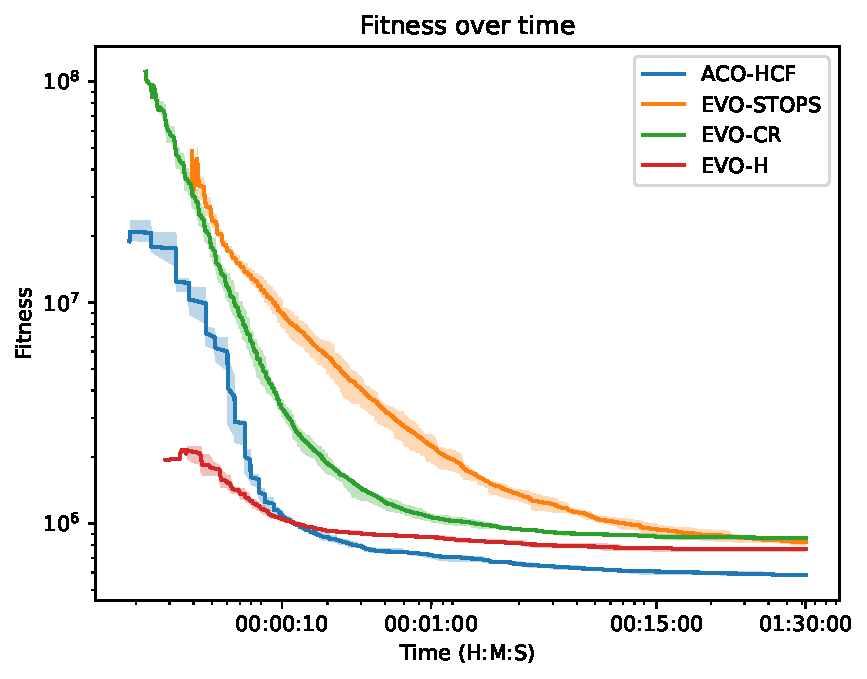
\includegraphics[width=1\linewidth]
    {img/exp_random_25b_100_time.pdf}
    \caption{Uniformly distributed dataset, 25 buses limit - Fitness values in time}
    \label{fig:exp_random_25}
\end{figure}

\begin{table}
    \centering
    \begin{tabular}{lcccccc}
         & Total costs & Distance traveled & Delay penalties & Buses used \\
         \hline
         EVO-STOPS & 732 & 2698 km & 18.9 (2\%) & 19 \\
         EVO-CR & 807 & 2458 km & 1.3 (0\%) & 22 \\
         EVO-H & 718 & 2459 km & \textbf{0.9 (0\%)} & 19 \\
         ACO-HCF & \textbf{566} & \textbf{2431 km} & 14.6 (3\%) & \textbf{14}
    \end{tabular}
    \caption{Uniformly distributed dataset, 25 buses limit - Route statistics}
    \label{tab:exp_random_25_route_stats}
\end{table}

\begin{table}
    \centering
    \begin{tabular}{lcccccc}
         &  Maximum delay & Average delay & Median delay \\
         \hline
         EVO-STOPS & 13m26s & 35s & \textbf{0s} \\
         EVO-CR & 4m18s & 7s & \textbf{0s} \\
         EVO-H & \textbf{3m52s} & \textbf{5s} & \textbf{0s} \\
         ACO-HCF & 11m54s & 41s & \textbf{0s} \\
    \end{tabular}
    \caption{Uniformly distributed dataset, 25 buses limit - Delay statistics}
    \label{tab:exp_random_25_delay_stats}
\end{table}

\clearpage

\begin{figure}
    \centering
    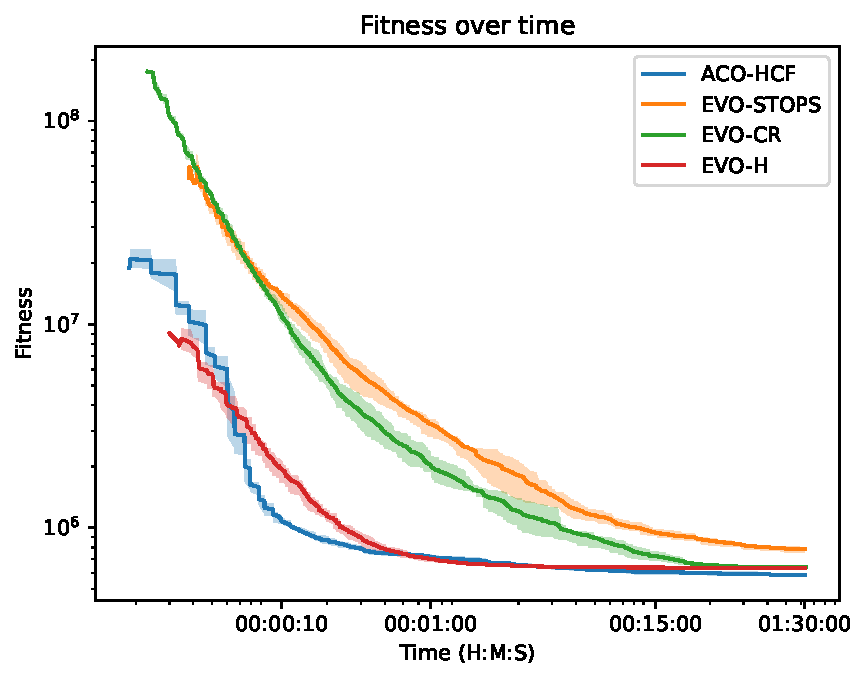
\includegraphics[width=1\linewidth]
    {img/exp_random_16b_100_time.pdf}
    \caption{Uniformly distributed dataset, 16 buses limit - Fitness values in time}
    \label{fig:exp_random_16}
\end{figure}

\begin{table}
    \centering
    \begin{tabular}{lcccccc}
         & Total costs & Distance traveled & Delay penalties & Buses used \\
         \hline
         EVO-STOPS & 635 & 2577 km & 108 (15\%) & 16 \\
         EVO-CR & 626 & 2440 km & \textbf{6 (1\%)} & 16 \\
         EVO-H & 597 & 2443 km & 9 (1\%) & 15 \\
         ACO-HCF & \textbf{566} & \textbf{2431 km} & 15 (3\%) & \textbf{14} \\
    \end{tabular}
    \caption{Uniformly distributed dataset, 16 buses limit - Route statistics}
    \label{tab:exp_random_16_route_stats}
\end{table}

\begin{table}
    \centering
    \begin{tabular}{lcccccc}
         &  Maximum delay & Average delay & Median delay \\
         \hline
         EVO-STOPS & 28m15s & 2m12s & \textbf{0s} \\
         EVO-CR & \textbf{8m19s} & \textbf{23s} & \textbf{0s} \\
         EVO-H & 8m33s & 30s & \textbf{0s} \\
         ACO-HCF & 11m54s & 41s & \textbf{0s} \\
    \end{tabular}
    \caption{Uniformly distributed dataset, 16 buses limit - Delay statistics}
    \label{tab:exp_random_16_delay_stats}
\end{table}

\clearpage

\subsection{150 customers}

For 100 customer requests over a 5-hour time window, the solutions ended up looking more like a taxi service instead of utilizing the advantages of bus transport. To avoid this, we created a larger and denser dataset, with 150 different requests during a 2-hour period. The bus type used is the same as in the previous dataset. We also doubled the computation time to 3 hours.

When using the \textit{ACO} approach, there is no direct way to limit the number of buses used, only by changing the delay penalty in the fitness function. In all \textit{GA} approaches, we limited the number of buses to $25$ to force them to utilize the buses. Therefore, the solution returned by the \textit{ACO} is not directly comparable to the other returned solutions.

The \textit{ACO} algorithm found a solution that uses $40$ buses. The characteristics of the solution remain the same as in the previous dataset. There are never 2 different customer groups on a bus at once, and the median delay is still 0. Both the total costs and distance traveled are, therefore, the highest. However, it minimized the fitness function the most. 

The best solution with a limited number of available buses was found by \textit{EVO-H}, with both total costs and customer delays better than in solutions found by \textit{EVO-STOPS} and \textit{EVO-CR}. \textit{EVO-STOPS} converged to a strictly worse solution, while also using a bus more (see ~\ref{evostops-catchroute}). \textit{EVO-CR} failed to converge in 3 hours and probably could have found a better solution if it ran longer. This makes \textit{EVO-H} a better choice for larger datasets.

We can also compare the results with the greedy heuristic approach described in~\ref{experiments-greedy}. When we run it with a maximum delay of 30 minutes, the travel time weight equal to $100$ a time violation weight equal to $1$, we get a solution that uses 42 buses, costs almost 1500k and travels for 3750km. The average delay is 8 minutes and 17 seconds. So \textit{ACO} found a solution with similar total costs, but smaller customer delays, while \textit{EVO-H} found a much cheaper solution with similar customer delays.

\clearpage

\begin{figure}
    \centering
    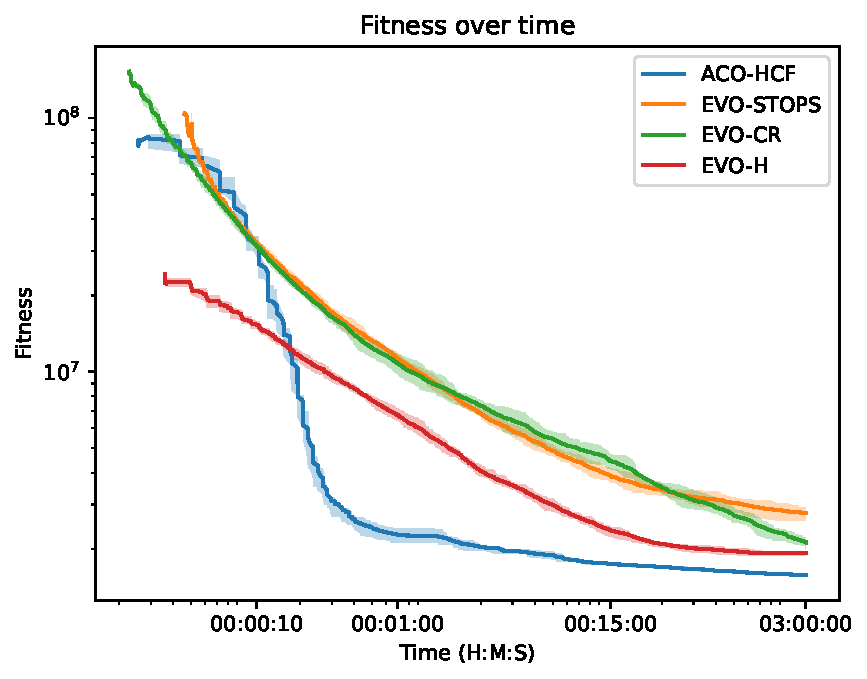
\includegraphics[width=1\linewidth]
    {img/exp_random_dense.pdf}
    \caption{Uniformly distributed dataset, dense data - Fitness values in time}
    \label{fig:exp_random_dense}
\end{figure}

\begin{table}
    \centering
    \begin{tabular}{lcccccc}
         & Total costs & Distance traveled & Delay penalties & Buses used \\
         \hline
         EVO-STOPS & 963 & 3049 km & 1585 (62\%) & 26 \\
         EVO-CR & 921 & 2850 km & 971 (51\%) & \textbf{25} \\
         EVO-H & \textbf{919} & \textbf{2822 km} & \textbf{905 (50\%)} & \textbf{25} \\
         ACO-HCF & 1427 & 3779 km & 128 (8\%) & 40 \\
    \end{tabular}
    \caption{Uniformly distributed dataset, dense data - Route statistics}
    \label{tab:exp_random_dense_route_stats}
\end{table}

\begin{table}
    \centering
    \begin{tabular}{lcccccc}
         &  Maximum delay & Average delay & Median delay \\
         \hline
         EVO-STOPS & 48m36s & 13m4s & 9m21s \\
         EVO-CR & 38m38s & 10m11s & 9m22s \\
         EVO-H & \textbf{36m56s} & \textbf{9m30s} & 7m25s \\
         ACO-HCF & 23m7s & 2m16s & \textbf{0s} \\
    \end{tabular}
    \caption{Uniformly distributed dataset, dense data - Delay statistics}
    \label{tab:exp_random_dense_delay_stats}
\end{table}

\clearpage

\section{Combined dataset}

Finally, we combined both types of requests in a \textit{combined dataset}. Approximately half of the
$100$ customers travel between Prague and Pilsen, while the other half travels either within Pilsen or Prague. Departure times are distributed randomly within a 4-hour time window. The available bus type has a capacity of $80$ persons, its operating cost per kilometer is $80$, and its fixed cost for rental is $50000$. The upper limit for buses used for genetic algorithms was set to $20$. The wall time was set to $120$ minutes.

The performance of each algorithm reflects its performance in both previous datasets. The \textit{ACO} performed the worst. When inspecting the best solution returned, it can be seen that the algorithm had the most trouble with the commute requests, most of the time failing to pick up multiple customers before traveling between the cities. This resulted in the highest number of buses used. However, it performed well with the requests within each of the cities, with the median delay being zero seconds. The genetic algorithms then performed surprisingly similarly. \textit{EVO-CR}
managed to lower the total costs the most, while \textit{EVO-H} dealt the best with group delays. Both of the algorithms have the same maximum delay, which belongs to the same group.

\clearpage

\begin{figure}
    \centering
    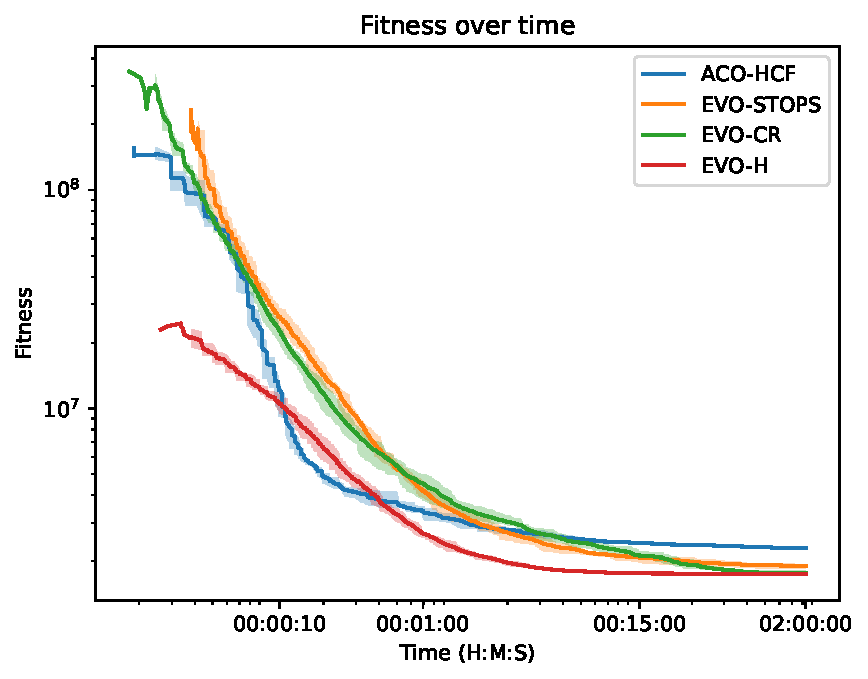
\includegraphics[width=1\linewidth]
    {img/exp_mixed_100_time.pdf}
    \caption{Mixed dataset - Fitness values in time}
    \label{fig:exp_mixed}
\end{figure}

\begin{table}
    \centering
    \begin{tabular}{lcccccc}
         & Total costs & Distance traveled & Delay penalties & Buses used \\
         \hline
         EVO-STOPS & 1597 & 6833 km & 219 (12\%) & 21 \\
         EVO-CR & \textbf{1522} & \textbf{6528 km} & 194 (11\%) & 20 \\
         EVO-H & 1529 & 6613 km & \textbf{159 (9\%)} & \textbf{20} \\
         ACO-HCF & 2060 & 9501 km & 174 (8\%) & 26 \\
    \end{tabular}
    \caption{Mixed dataset - Route statistics}
    \label{tab:exp_mixed_route_stats}
\end{table}

\begin{table}
    \centering
    \begin{tabular}{lcccccc}
         &  Maximum delay & Average delay & Median delay \\
         \hline
         EVO-STOPS & \textbf{21m23s} & 5m15s & 3m18s \\
         EVO-CR & 21m47s & 4m43s & 2m6s \\
         EVO-H & 21m47s & \textbf{2m5s} & 15s \\
         ACO-HCF & 34m11s & 2m50s & \textbf{0s} \\
    \end{tabular}
    \caption{Mixed dataset - Delay statistics}
    \label{tab:exp_mixed_delay_stats}
\end{table}

\clearpage